\documentclass[pageno]{jpaper}

%replace XXX with the submission number you are given from the ISCA submission site.
\newcommand{\IWreport}{2015}
\newcommand{\project}{IMAPSec }

\usepackage[normalem]{ulem}
\usepackage{listings}
\lstset{language=Python}

\begin{document}


\title{Making (Secure) FETCH Happen:
\\ \vspace{2 mm} {\large Providing End-to-End Metadata Security for IMAP}}

%  Providing End-to-End Metadata Security for IMAP
% \title{\project: Secure, Backwards-Compatible Storage for Metadata-Secure Messaging Systems
% \\ \vspace{2 mm} {\large Invisibly Protecting Content and Metadata On Johnny's Behalf}}

\author{Erica Portnoy}

\date{}
\maketitle

\thispagestyle{empty}

\tableofcontents

\begin{abstract}
Email, but metadata and content are E2E encrypted. No usability concessions. A non-technical user will have no more trouble using it than they would with https vs. http. Departure from classical message encryption usability theories in that it places no burden on the user.
\end{abstract}

\section{Introduction}
% Background information and problem description. What is the general area of research and the specific problem that will be tackled?

One, a Hard Problem in Secure Communication is metadata \cite{hardprob}. Two, usable encryption tools for email is historically hard and still is \cite{johnny}. But https does it just fine. Goal: develop the necessary ecosystem to enable metadata-secure email with no extra effort from the end user.

Give a history of email security/usability/etc. PGP, Why Johnny can't encrypt \cite{johnny}, iMessage, TextSecure and WhatsApp. Introduce the term metadata-secure messaging (MSM).

\section{Related work}
% Related research. Have there been previous academic papers on this or related topics? Are there companies that have developed related software products? What is the historical context? Be sure to cite related research properly. Include a bibliography at the end of your paper.
Many combinations of options exist \cite{spreadsheet}. (Figure out how to cite JB's Summary of Knowledge.)

\subsection{Facebook Message Hannover Study}
What I'm working on for email, but for Facebook. \cite{fahl}

\subsection{Email over Tor}
Tor Mail, OnionMail

\subsection{Mailpile}
Their general ideas, storage solutions. \cite{mailpile}

\subsection{Mailpile SMTorP Plugin}
Explain Tor \cite{tor}, .onion Addresses \cite{smtorp}

\subsection{Pond}
Pond is a system for forward secure asynchronous messaging that does not leak traffic information ``except [to] a global passive attacker." \cite{pond}

Through these tools, the transport mechanism becomes more secure. Yet for all of these, messages are assumed to be transient or remain only on the client device. This is unacceptable behavior to a typical modern user. Modern users expect their emails to be stored on a server and available to them from multiple clients -- from their computers, mobile devices, and on the Web. To ubiquitize secure email, we must develop a storage and synchronization solution that protects messages at rest without compromising the benefits of secure transport protocols.

\section{Threat Model}
Use trike.

\section{Target User}
\label{targetuser}

\section{Design Goals and Non-Goals}
\label{goals}

Some discussion of the usability issues. Garfinkel et al. \cite{garfinkel} talk about ``How to make secure email easier to use,'' and Ruoti et al. talk about dangers in automatic encryption \cite{ruoti}.

\section{Relevant Email Technologies}
Explain how SMTP and IMAP legacy versions work. Probably with some diagrams!
\subsection{Mail Sending and Transport}
SMTP

\subsection{Mail Retrieval, Storage, and Synchronization}
\subsubsection{POP}
\subsubsection{IMAP}
IMAP uses a command-response model. Commands are either tagged with OK, BAD, or NO, or untagged.

\label{legacyimap}


\section{Architecture and Data Flow}
\label{architecture}
% Have you defined your overall software architecture? -- describe it in detail and justify your design.

As discussed in Section~\ref{goals}, a permissible \project solution must be built to integrate with legacy systems. An MSM MUA will also accept legacy SMTP traffic, and it must appear to the user that all messages, once received, are the same. While the user experience must remain consistent, there are multiple possibilities for architecting a storage system consistent with the storage needs. To architect such a backend, there are several possibilities:

\begin{enumerate}
	\item Keep all messages on the local machine only.
    \item Store messages in a secure, remote, user-controlled filesystem.
    \item Use the infrastructure of existing IMAP servers.
\end{enumerate}

The first is unacceptable, given the target user group described in Section~\ref{targetuser}, as this would violate user expectations. To implement the second, we would need to describe a server infrastructure for storing messages and synchronizing across multiple possible clients who have subscribed to updates on messages stored in the system -- which is to say, (a subset of) the functions that the IMAP server is designed to perform. This brings us to our final option, using a modified version of existing IMAP technology, which was described in Section~\ref{legacyimap}.

In the \project protocol, a standard IMAP client library is wrapped with a \project module. An MUA then uses the \project module in lieu of a standard IMAP connection agent. This module will perform all necessary functions on behalf of the MUA, including encryption, UID translation, and metadata tracking.
% The \project protocol is 
% The core elements of the \project protocol are 
% \begin{enumerate*}[label=(\itshape\arabic*\upshape)]
% \item an \project module used in lieu of a standard IMAP connection agent in an MUA, and
% \item an index file that is stored as a regular message in a legacy IMAP server. \end{enumerate*}
As further described in later sections, the module ensures that metadata is encrypted along with message contents for all messages to be stored on the IMAP server. It also handles the indexing functions, mapping mailboxes to the messages they complain. This is a significant departure from the legacy system, where mailbox names and contents were exposed to the IMAP server. As such, it shifts the burden of tracking, updating, and syncing changes to the INDEX from the server to the client. When one client updates the INDEX, the IMAP server will see that a message has changed, and inform its other clients in the standard method. 

% Such updates may arise from moving messages between mailboxes as they appear to the client to exist, necessitating careful bookkeeping of the index file.

Note that these changes imply that if one client of an IMAP server is \project-compliant, all clients subscribed to that server must also be \project-compliant. Otherwise, all other clients will see only the encrypted messages as the IMAP server would see them; this is a necessary and desirable feature of the system.

These changes permit the combination of MSMs and non-MSMs in the same storage system, ensuring an elegant transition to a more secure email.

\label{mail-from-secure}
\subsection{Mail From a Secure Source}
When email is received from a metadata-free source (SMTorP, DIME, Pond, etc.), it is stored in a ``cryptoblobs'' mailbox on the IMAP server that the client's \project module has set up. This change is then marked in the INDEX, which is correspondingly updated.

  \begin{tikzpicture}[node distance=2.5cm]
  \node (alice) [box] {Alice};
  \node (smtpa) [box, above of=alice] {Alice's metadata-\\ secure server};
  \node (cloud) [cloud, draw,cloud puffs=10,cloud puff arc=120, aspect=2, inner ysep=1em, right of=smtpa, xshift=1.3cm] {Network};
  \node (imapb) [box, right of=cloud, xshift=1.3cm] {Bob's metadata-\\secure server};

  \node (bob) [box, below of=imapb] {Bob\\
  \trimbox{0cm 0cm 0cm -.2cm}{
  \begin{tikzpicture}
  \node (imaps) [box, minimum height=.5cm, outer sep=.2] {\project module};
  \end{tikzpicture}}};
  \node (bobimap) [box, right of=imapb, xshift=1cm] {Bob's legacy \\ IMAP server \\ \trimbox{0cm 0cm 0cm -.2cm}{
  \begin{tikzpicture}
  \node (index) [box, minimum height=.5cm, outer sep=.2] {INDEX};
  \end{tikzpicture}
  } };

  \draw [arrow] (alice) -- (smtpa);
  \draw [arrow] (smtpa) -- (cloud);
  \draw [arrow] (cloud) -- (imapb);
  \draw [arrow] (imapb) -- (bob);
  \draw [arrow] (bob) -| (bobimap);

  \end{tikzpicture}


\label{mail-from-insecure}
\subsection{Mail From an Insecure Source}
When an email is received through (legacy) SMTP, it is deleted from the server, its contents and metadata encrypted, and reuploaded to the IMAP server in the same way as an email that was received from a secure source.

  \begin{tikzpicture}[node distance=2.5cm]
  \node (alice) [box] {Alice};
  \node (smtpa) [box, above of=alice] {Alice's legacy \\ SMTP server};
  \node (cloud) [cloud, draw,cloud puffs=10,cloud puff arc=120, aspect=2, inner ysep=1em, right of=smtpa, xshift=1.3cm] {Network};
  \node (imapb) [box, right of=cloud, xshift=1.4cm] {Bob's legacy \\ IMAP server \\
      \trimbox{0cm 0cm 0cm -.2cm}{
          \begin{tikzpicture}
              \node (index) [box, minimum height=.5cm, outer sep=.2] {INDEX};
          \end{tikzpicture}
      } 
    };

  \node (bob) [box, below of=imapb] {Bob\\
    \trimbox{0cm 0cm 0cm -.2cm}{
    \begin{tikzpicture}
            \node (imaps) [box, minimum height=.5cm, outer sep=.2] {\project module};
        \end{tikzpicture}}};

  \draw [arrow] (alice) -- (smtpa);
  \draw [arrow] (smtpa) -- (cloud);
  \draw [arrow] (cloud) -- (imapb);
  \draw [arrow] (imapb.260) -- (bob.103);
  \draw [arrow] (bob.77) -- (imapb.280);

  \end{tikzpicture}
  

\section{Email Usage Measurements}
To determine various factors such as how often to update and how large a fake message should be, an implementation of \project should measure and dynamically learn these values for actual incoming messages for each particular user. The usage patterns of a typical American college student are as follows.

\subsection{Size}

Email sizes follow a ``long tail" logarithmic distribution. Sizes below are calculated on a mailbox with a total of 77002 messages.

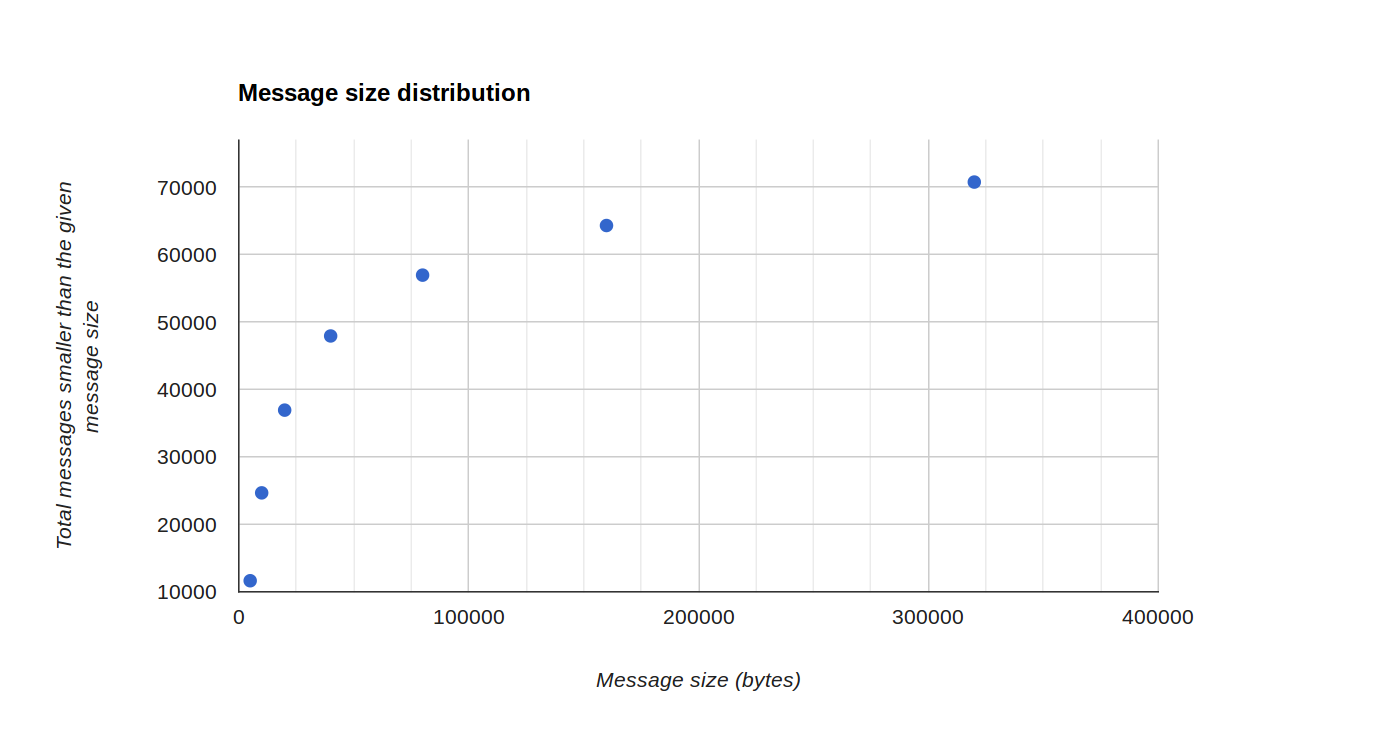
\includegraphics[width=\textwidth]{message-size-dist}

\subsection{Timing}
  
\section{Technical Details}

\label{initialization}
\subsection{Initialization}
Upon logging into an IMAP server, \project attempts to select the CRYPTOBLOBS mailbox. If it succeeds, it assumes that this server has been previously initialized by itself or another client. If there is no CRYPTOBLOBS mailbox, it creates one. It then generates a random salt, appends an initial INDEX with SEQUENCE NUMBER 1 and the salt in the subject line of the INDEX, appends a LOCK, and fetches and loads the INDEX.

\subsection{Command Translations}
The \project module sits between the client and the legacy IMAP module. It translates arguments, processes data, and returns results that give the client a pseudo-view of the contents of the IMAP server informed by the contents of the metadata INDEX. There are four possible mailbox classifications. The classification determines the actions that the module takes in response to each command. A PSEUDO mailbox is not mirrored in the IMAP server; it exists only in the INDEX and is thus only known to clients following the \project protocol. A HYBRID mailbox exists both in the IMAP server and in the INDEX. This is a mailbox such as INBOX, which must also be known the IMAP server as a location for the delivery of incoming messages. A PSEUDO/HIDDEN mailbox neither exists in the IMAP server nor is known to the client. It is for use only by the \project module. The FAKE\_MESSAGES mailbox used by the scheduler is an example of this type of mailbox. An ACTUAL/HIDDEN mailbox is known to the IMAP server but not to the \project client. The CRYPTOBLOBS mailbox, the mailbox in which all encrypted messages are stored on the IMAP server, is an example of this type of mailbox. 

\label{select}
\subsubsection{SELECT} In a view of the system enforced by the Python wrapper for an imap connection, imaplib, when a SELECT command is passed to the IMAP module, the state of the IMAP server changes to record that a particular client connection has selected a mailbox, and returns a count of the number of messages in that mailbox. When the \project module receives a SELECT command, it saves the requested mailbox to an instance variable. If the requested mailbox is a HYBRID mailbox, it passes the count onto the IMAP server. For both PSEUDO and HYBRID mailboxs, it then calculates the number of messages in the mailbox based on the INDEX, and adds that to either the returned value or 0. If a HIDDEN mailbox is requested, a NO response is returned. Note that the counting functionality is implemented by the EXISTS untagged request as described in Section~\ref{exists} - the SELECT command elicits the EXISTS server response, whose value is used for the return value of the Python function.

\subsubsection{FETCH} A FETCH or UID FETCH command requests information about a particular message, including either metadata or a subset of message body contents. For both metadata and body, \project first translates the requested UID as described in Section~\ref{uid-translation}. If it is a metadata request, it then forwards the translated command to the IMAP server, and uses the response from the server. Note that metadata here means the metadata the IMAP server uses to keep track of its messages, namely FLAGS, INTERNALDATE, RFC822.SIZE, and ENVELOPE. If it is a body request, \project requests the entire message body (body here includes headers). It then checks that the hash matches, as further described in Section~\ref{rollback}. It then decrypts and checks the authentication of the message, as described in Section~\ref{encryption}. Finally, it returns the appropriate components as specified in the initial request.


Note that the present prototype implements only a subset of FETCH commands. Particularly, only metadata or the entire body can be requested. This is sufficient for use with the prototype's client, Mailpile.

\subsubsection{SEARCH} A SEARCH command acts on the selected mailbox. Similarly to SELECT handling as described in Section~\ref{select}, \project returns results from HYBRID and PSEUDO mailboxs as appropriate. The current version of the prototype only responds to SEARCH ALL commands, which list all UIDs in the mailbox in ascending order. By RFC 3501, the IMAP specification, a SEARCH command should handle a wide variety of requests. Many of these would require iterating through each message in the pseudo-mailbox, or searching on encrypted data. While one could imagine protocols for constructing efficient indexes or incorporating homomorphic encryption, that is beyond the scope of this project.

\subsubsection{FLAGS} The FLAGS command is called for a specific mailbox, to ask which flags are valid inside that mailbox. Since the prototype client neither sets nor checks any message FLAGS itself, \project merely responds with the flags for the INBOX mailbox. A full implementation would allow flags to be set for individual messages within the metadata INDEX, largely reimplementing the IMAP server storage functionality on the client-side using the INDEX.

\subsubsection{UIDVALIDITY} UIDVALIDITY is a mechanism for detecting non-persistence of message UIDs. \project does not allow UIDs to change over time, so as per the RFC, we may return `1' for any mailbox where we are handling UIDs \cite{rfc3501}.

\label{exists}
\subsubsection{EXISTS} EXISTS is functionally equivalent to the return value of SELECT. The technical definition is the number of messages in the mailbox.

\subsubsection{RECENT} RECENT is requested but ignored by the prototype client, so we return `0'.

\subsubsection{LIST} The LIST command is used to recursively find all mailboxes in the server. The current prototype allows only top-level, no-children PSEUDO mailboxes. Thus, in translating LIST results, \project inserts PSEUDO mailbox results as if they were to exist at the top level. \project also removes HIDDEN folders from the LIST results before returning.

\label{uid-translation}
\subsection{UID Storage and Lookup}
While all encrypted messages are stored on the IMAP server in the CRYPTOBLOBS mailbox, the client's view should allow for a more complex representation of which messages are stored in which mailboxes. At a minimum, we would like to support an INBOX mailbox for messages that are received at the IMAP server, and an SMTorP or Pond folder for messages that are received at the client via a metadata-secure transport mechanism. Thus, each message needs an associated UID for its pseudo-mailbox, or the mailbox that the message is in as it appear to the client. But it also has an actual UID, or the UID inside the CRYPTOBLOBS mailbox. This UID is assigned by the IMAP server when \project APPENDs a message to a mailbox on the server. The APPEND command does not, however, return the assigned UID. Therefore we need a separate mechanism for associating a message's pseudo-UID with its actual UID.

To handle this, before appending a message to CRYPTOBLOBS, \project generates a 16-byte random UNIQUE SUBJECT number. This number is placed in the subject line of the appended message, forming an full subject line of the form ``ENCRYPTED <UNIQUE SUBJECT>". Then, when the client requests a message via a specific mailbox/UID pair, \project uses the INDEX to look up the UNIQUE SUBJECT for the pseudo-UID in the appropriate mailbox. It then searches for the message in CRYPTOBLOBS with UNIQUE SUBJECT in its subject line, which returns the unique actual UID of the message in the CRYPTOBLOBS mailbox.

For example, say the INDEX contains the following entry:

\begin{lstlisting}
INDEX = {`INBOX':{`36':`006a033f49f579f9a36e9afcfb1e7747'...}...}
\end{lstlisting}

If the client wished to acquire this message, it would issue the following commands:

\begin{lstlisting}
SELECT INBOX
UID FETCH 36 <REQUEST>
\end{lstlisting}

This would issue a request for message 36 in mailbox INBOX. \project would then note that
the UNIQUE SUBJECT for 36 in INBOX is 006a033f49f579f9a36e9afcfb1e7747, and issue the following requests to the server:

\begin{lstlisting}
SELECT CRYPTOBLOBS
SEARCH SUBJECT 006a033f49f579f9a36e9afcfb1e7747
\end{lstlisting}

This would return a list of all UIDs of messages with 006a033f49f579f9a36e9afcfb1e7747 as a substring of the subject in mailbox CRYPTOBLOBS. Since this is a 16-byte number, there is only a $1/2^{128}$ chance of two messages having the same UNIQUE SUBJECT, so this SEARCH will probably return only a single UID:

\begin{lstlisting}
OK 129
\end{lstlisting}


\project, now knowing the actual UID, can then issue the following request to the server:

\begin{lstlisting}
UID FETCH 129 <REQUEST>
\end{lstlisting}

One potential optimization here would be to perform the SEARCH immediately after each APPEND. The utility of this optimization is based on the number of subscribed clients and the probability of being selected to be pulled down in a mix. That is, if more than one FETCH will occur per APPEND, then it may make sense to cache the actual UID in the index.

\label{processing}
\subsection{Processing Messages Received at IMAP Server}
When a message is received at the IMAP Server as in Section~\ref{mail-from-insecure}, \project processes the message so it is equivalent to messages that arrived at the client machine from a secure source. To process a message, \project fetches the body of the message, adds it to CRYPTOBLOBS, and deletes it from the INBOX. Note that without any mixing here or during scheduled message exchanges, it is trivial for an IMAP server to keep track of which message in CRYPTOBLOBS corresponds to which message that was received in the INBOX, because the server will see that a message was added to CRYPTOBLOBS and deleted from INBOX at about the same time. The process used for adding the message to CRYPTOBLOBS is equivalent to the process for adding a message from an insecure source, or for adding a scheduled fake message. The process for adding a message to a pseudo-mailbox involves several steps. We update the INDEX, possibly adding the mailbox to the INDEX if it is the first time we have seen it. We generate a UNIQUE SUBJECT number. If the mailbox is of type PSEUDO, we compute the pseudo-UID for the message. As per RFC 3501, the UID assigned is strictly greater than any UID that has been previously assigned in the mailbox. We store in the INDEX the state of the NEXT UID to assign.


\subsection{Multiple Client Synchronization and Concurrency}
Central to IMAP's design is the ability to handle the actions of multiple clients subscribed to the server. The core synchronization feature is the INDEX. Since it resides in the CRYPTOBLOBS folder that all IMAP clients have access to, any client will see the updates to the INDEX made by any other client. Some actions need only be completed by one client though, such as those described in Sections~\ref{initialization} and \ref{processing}. These will be handled by the first client to notice the preconditions for those actions, namely an uninitialized IMAP server or a message in the actual INBOX mailbox.

Given the structure of the IMAP commands, there is no drawback to being either the first or a later client to perform the action. For example, a client of \project that asks how many messages are in the INBOX will be returned the same number in response to a SELECT whether they were the one to process an incoming message or not, and will be returned the same list of pseudo-UIDs in response to a SEARCH ALL.

Some \project actions must be atomic, namely the coupling of appending and deleting messages from mailboxes with fetches of and updates to the INDEX. \project solves this via a LOCK mechanism. A message with SUBJECT line LOCK is deleted from and appended to the CRYPTOBLOBS mailbox to acquire and release a lock, respectively.

Because of this delete/upload lock acquisition mechanism, the IMAP server may sometimes be in a state where the LOCK message does not exist but no client holds the lock, such as if a client crashes or closes down while holding the lock. Optimally, this would not happen, and the lock would be released before closing, but the existing library does not require a method to be called on close, so we cannot rely on a client to release a lock before quitting. Thus, \project includes a mechanism for detecting this inconsistent state and recovering from it by acquiring a lock even if the LOCK message does not exist in the CRYPTOBLOBS mailbox.

The lock recovery mechanism waits until a specified time (default 60 seconds), checking for the existence of the lock every few (default 2) seconds within that interval. After the time is completed, \project attempts to fetch the INDEX. If the index is not there, we assume that another client has failed and acquire the lock ourselves. If the index is there but has not been updated during that time (using the SEQUENCE NUMBER to determine this), we again acquire the lock. Yet if the index is there and has been updated, we assume someone else is still using the lock and double the total wait time until our next check.

\subsection{Deletion}
Various \project actions include deletion of a message from the CRYPTOBLOBS mailbox. In general, not deleting a message will not leak any data to the IMAP server, since our threat model includes a server than can either refuse to delete or can save a backup version of any message. Yet for practical reasons such as mailbox data usage and lack of clutter, it is generally beneficial to at least attempt to delete a message. Here we must note that IMAP servers may differ in their implementation in regard to the location of messages, potentially complicating deletion protocols. For example, Gmail uses its All Mail mailbox (``label'', in their terms) as a message archive \cite{allmail}. That is, if a message appears in any mailbox, it will also appear in the All Mail mailbox. If it is deleted from All Mail but still exists elsewhere, it will be replaced in All Mail. Thus, to delete a message from any non-All Mail mailbox, it must first be deleted from all other mailboxes then deleted from All Mail. Note that the message will be assigned a different UID for each mailbox that it appears in.

Deleting a message that has already been processed is simple; we may use UNIQUE SUBJECT as in Section~\ref{uid-translation} to find the message in any mailbox, including All Mail. For a message that has arrived in the INBOX though, we must be more careful. To delete such a message from All Mail, we must first search for it (by subject or otherwise), then test all resulting UIDs for exact message equivalence to the message that we intend to delete from the non-All Mail mailbox.

\subsection{INDEX Caching}

\section{Security}

\label{encryption}
\subsection{Encryption}

When a message is appended to the CRYPTOBLOBS mailbox, whether it be a processed INBOX message, a fake message created on schedule, or a message from a metadata-secure source, it is encrypted before being uploaded. It is encrypted using the standard method of authenticated encryption, which is to say that a Message Authentication Code calculated on the encrypted message is concatenated to the encrypted message. Data is encrypted using AES-CBC and signed with HMAC-SHA256. The encryption key is derived from the random salt created during initialization (as described in Section~\ref{initialization}) and a passphrase using scrypt \cite{percival2009stronger}. Scrypt is a memory-hard key derivation function that imposes a cost for deriving a key given a guess of a passphrase by using many sequential iterations that cannot be parallelized on specialized hardware.

The passphrase is passed into the \project module at runtime initialization of the class. This leaves handling of the passphrase to the client. They can choose to ask the user for it on each initialization, ask once and save for future use, or a hybrid of the two methods. The user can choose a passphrase, or the client can generate a passphrase and instruct the user to save it. The latter method is currently not supported (although it could be), as it would require a mechanism for merely checking if the server has been initialized without initializing it. If the programmatically-generated passphrase method is used, we suggest displaying it as a ``backup code'' as in Yahoo!'s End-to-End Encryption Extension \cite{yahoo} for usability reasons; users are familiar with the concept of backing up data, but may not be as familiar with keys and passphrases.


\label{rollback}
\subsection{Rollback Detection}
While we cannot rely on the IMAP server for availability, we can detect and decline to accept rollback of any part of the system. Each time that the INDEX is updated by any client, its SEQUENCE NUMBER is incremented. Thus, when a new INDEX is downloaded, the \project module compares the SEQUENCE NUMBER of the received INDEX to the most recent SEQUENCE NUMBER. If the downloaded sequence number is not at least the value of the SEQUENCE NUMBER known to the client, then the new index is not accepted. It saves this in memory, but also stores it to a local file specified by the client of the module. When a client first connects to an IMAP server that has already been initialized, it uses the current INDEX's SEQUENCE NUMBER as the initial number.

Rollback detection for individual messages relies on the rollback detection of the INDEX. When a message is appended to CRYPTOBLOBS, its hash is saved in the INDEX along with its pseudo-UID and UNIQUE SUBJECT. Each time the message body is FETCHed, the body is hashed and compared to the saved hash. If they differ, then the message has been changed. Thus, if the INDEX is current (and since the INDEX is saved in the server under authenticated encryption), an adversary cannot replace the message with a version whose hash is not saved in the current INDEX.


\section{Protecting Metadata}

If a message has been received at the client from a secure source as in Section~\ref{mail-from-secure}, we would like to upload it to the IMAP server so that other \project clients can view it, and to achieve user-facing functionality backwards compatibility. Yet if we push a message to the server immediately upon its receipt, we are leaking the time of message receipt to the server. Thus, we need additional mechanisms for ensuring that a server that stores messages cannot determine when a message arrived.

\subsection{Scheduler: Delivering from IMAP Client to IMAP Server}
The primary mechanism for limiting the amount of data the server can determine regarding message arrive metadata is a scheduling module that determines when a message should be pushed up to or pulled down from the server.

  \begin{tikzpicture}[node distance=8cm]
  \node (\project) [box, minimum height=2cm] {\project};

  \node (scheduler) [box, minimum height=2cm, right of=\project] {Scheduler};

  \draw [arrow] (\project.10) -- node [above] {State information} (scheduler.-190);
  \draw [arrow] (scheduler.190) -- node [below] {Next action: UP/DOWN} (\project.-10);
 
  \end{tikzpicture}

This scheduler receives information from the \project module about its state. Namely, it is informed when a message is received at the client or marked for deletion on the server. Instead of immediately performing this action, the \project module will wait until the next timer tick, when it is called to perform its next scheduled action by its client. At that time, it asks the scheduler whether its next action is an UP or DOWN action. The scheduler considers how often messages are being received and how often scheduled communications happen, and returns an UP or DOWN result to keep overall server growth consistent with actual message receipt and deletion rates. The server will be able to see that an UP or DOWN has been performed on schedule, but will gain no more than one bit of metadata on every timer tick.

To implement this one-bit leakage, \project must either push up or pull down a message on each timer tick, whether or not it is has a message to deliver or a deletion scheduled. This condition is satisfied through artifically constructed messages. A constructed message with contents of a random size chosen from a distribution mirroring that of messages usually sent and received of the user is generated, encrypted and packaged as if it were a legitimate message, saved to a FAKE MESSAGES PSEUDO-mailbox, and sent to the server. On deletion, a message from FAKE MESSAGES is chosen at random and deleted in lieu of a legitimate message. These actions appear identical to the server, since the server will see only updates to the INDEX and the append or delete of a message with subject ENCRYPTED <UNIQUE SUBJECT> and encrypted contents.

Even if the user never deletes a message, the scheduler should still periodically return a DOWN bit, so that the contents of the server do not needlessly continuously grow at a high rate. In the case where deletes never occur, one could imagine a schedule of only pushes, timed such that is it similar to the actual receipt rate, say every 20 minutes. This is an unacceptable rate of checking for mail in a modern system, where periodic updates occur an order of magnitude faster. Additionally, since only one message is pushed every $t$ minutes, messages received in a batch of $k$ would be delayed at least $k*t$ minutes.

% Learning Update Schedules - Exponential backoff?

\label{mixing}
\subsection{Message Mixing}
The scheduling mechanism is necessary but not sufficient to hide message arrival metadata from the server. Assume a user never deletes messages, for simplicity. Assume also that the server is maliciously attempting to track metadata, and notes the upload time of each message. Consider two messages, R and F. R is a real message, and F a fake. Initially, the server cannot distinguish between the two messages. Since R is real, there is a probability $p=0$ that it will be deleted at any point in the future. The goal of the scheduling algorithm is to send messages to the server at an effective rate similar to the rate of actual message receipt, so the server does not grow needlessly. Then, the number of fake messages will remain about constant, $k$. So at each timer tick where a DOWN occurs, a fake message will have probability $p=1/k$ of being deleted. Therefore, the probability that a message is not deleted after $n$ DOWN ticks is $(1-1/k)^n$ (since it must not be deleted at all time ticks), which tends towards 0 as $n$ increases. Thus, a fake message's long-term probability of being deleted is 1. So, after a length of time has passed, any message that was uploaded to the server and has remained there for a long period of time is likely a real message, and the server can therefore merely observe the time it was uploaded.

This analysis does not only apply in the theoretical sense. Assume the user had let the system run in a mode where more fake messages are uploaded than are deleted until it was seeded with 5,000 fake messages. After that point, the user wants to keep the size of the mailbox constant, so for each upload (received message), they delete a message as well. Assume also that they would like to spread new messages to other clients of the server within 10 minutes of its receipt (a conservative estimate). Then they must delete a message every 10 minutes as well, which amounts to 144 deletions a day, 52,560 a year, and 262,800 in a five year period, which we conservatively assume is the length of time a user would like to keep an email account for. So $k=5000$ and $n=262800$, giving a probability of a fake message not being deleted of about $1.5\times10^{-23}$, which is certainly distinguishable from $p=1$ for a real message.

\subsubsection{Hiding Among Many}
We can imagine a solution to this problem where many more fake messages are added than real messages, driving down the probability that a fake message is chosen for deletion until it resembles the probability that a real message is chosen, 0. (Note that even in this case we will still desire scheduled deletions, to disguise deletions of real messages.) Assume for simplicity that fake messages are added at an amortized constant rate. We would like to calculate the probability that a fake message is not deleted after the $n$ DOWN ticks following its upload at time $t$. This is equal to the product of the probabilities that a fake message was not deleted at all ticks between times $t$ and $t+n$. We can compute this based on the probability of deleting a message at a particular time after $i$ deletion intervals. Assume that at each each interval, $c+1$ real messages and $f$ fake messages came in. Then the probability that a message was fake is $f/(c+f+1)$, and $c+f+1$ messages total came in each interval. But one message was deleted each interval, so $c+f$ net messages are added. So after $i$ intervals, $i(c+f)$ messages are in the server total, and an expected $i(c+f)f/(c+f+1)\approx if$ of those are fake. So the probability of a message being deleted at time $i$ given that it is fake is $1/(if)$, and the probability that it is not deleted is $1-1/(if)$. Then if the message was uploaded at time $t$, the probability that it was not deleted at time $n$ is $\displaystyle\prod_{i=t}^{i=t+n}(1-\frac{1}{if})$. This product tends towards 0 as $n$ tends towards infinity, but its slope drops off quickly as $f$ increases.

For example, consider the following graph of the probability of a message being not deleted from when it was added at time $i=250$, until time $i=1000$.

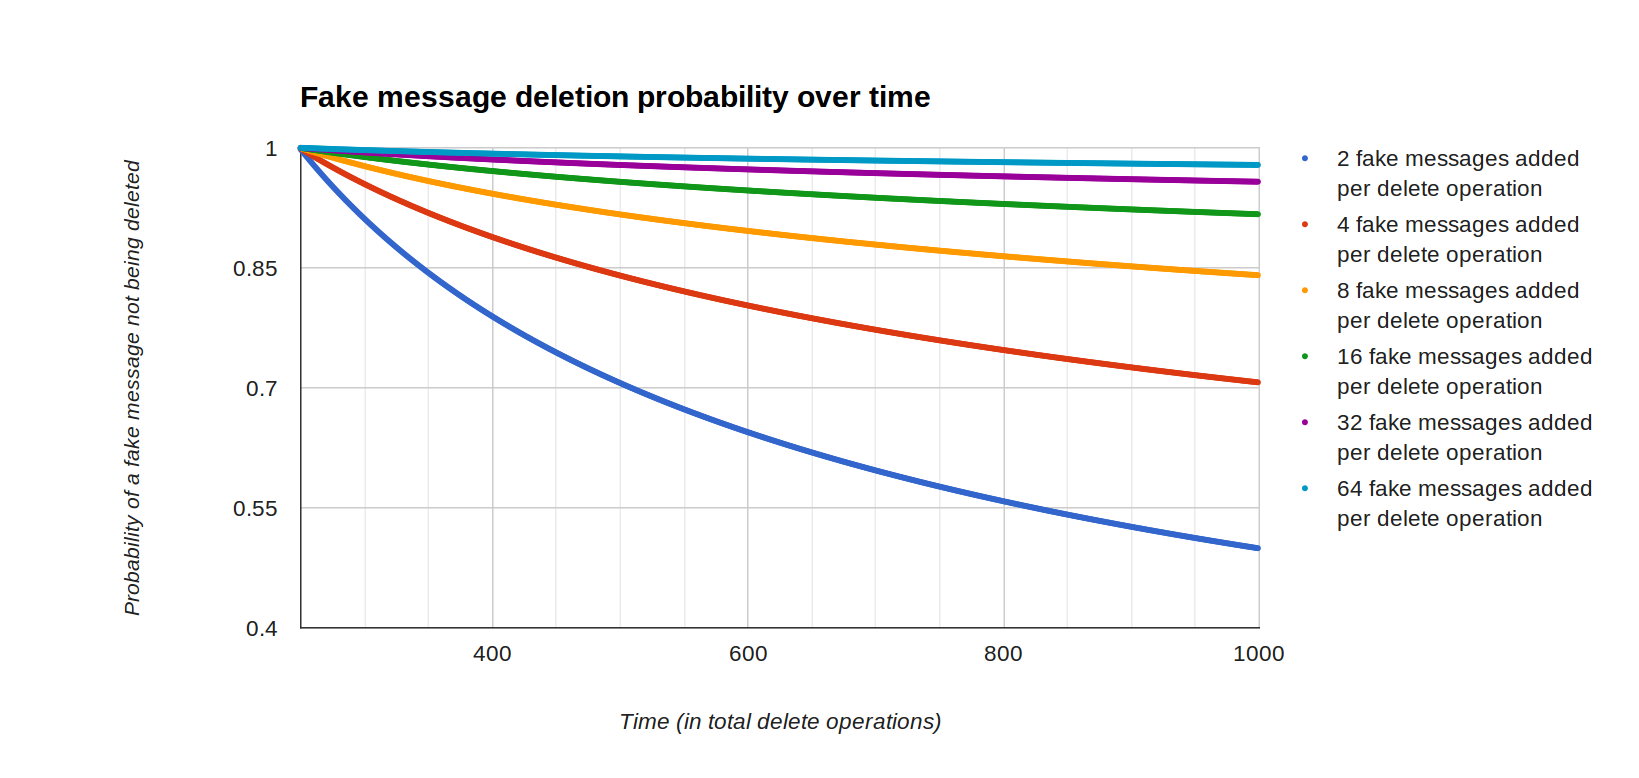
\includegraphics[width=\textwidth]{many_lines_2}

Note that if 32 or 64 messages are added per deletion operation, the probability that a fake message is not deleted remains at 0.96 and 0.98 even after $1000-250=750$ operations. This comparison is shown more clearly in the following graph.

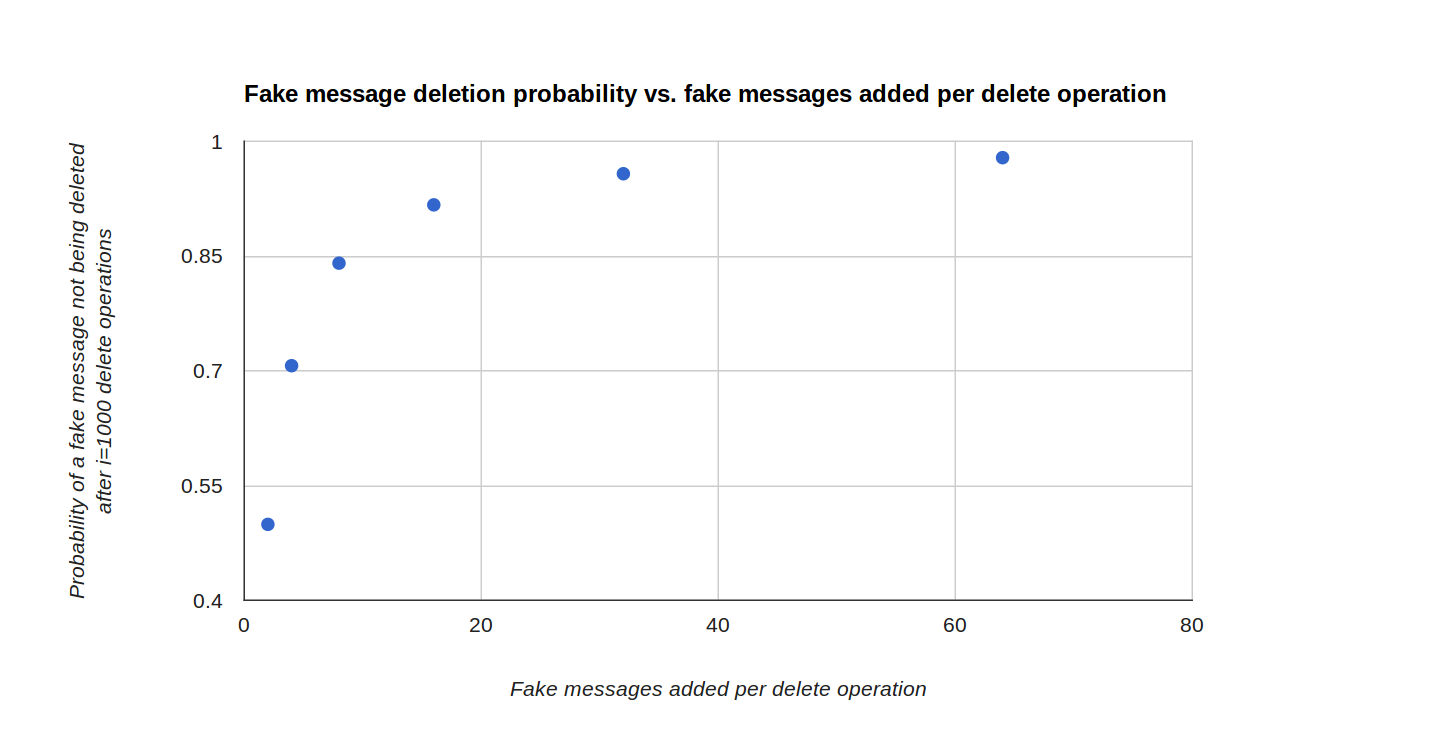
\includegraphics[width=\textwidth]{few-blue-dots-250}


Yet we only achieve these high rates after the server has been seeded with an adequate number of fake messages, as demonstrated by altering our parameters to show the results when a fake message is instead added at interval $i=0$.

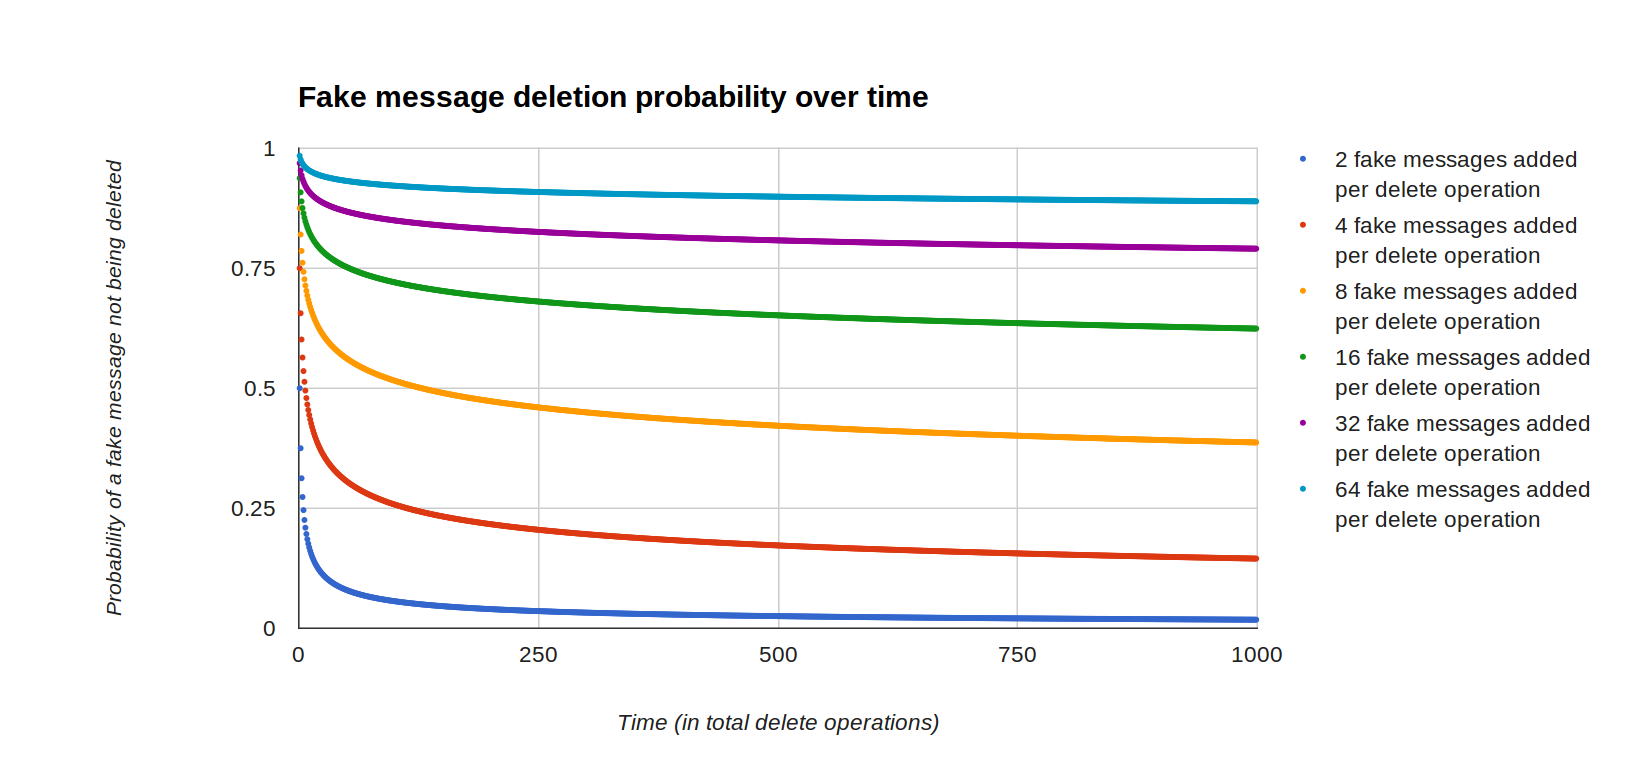
\includegraphics[width=\textwidth]{fake-message-deletion-over-time}

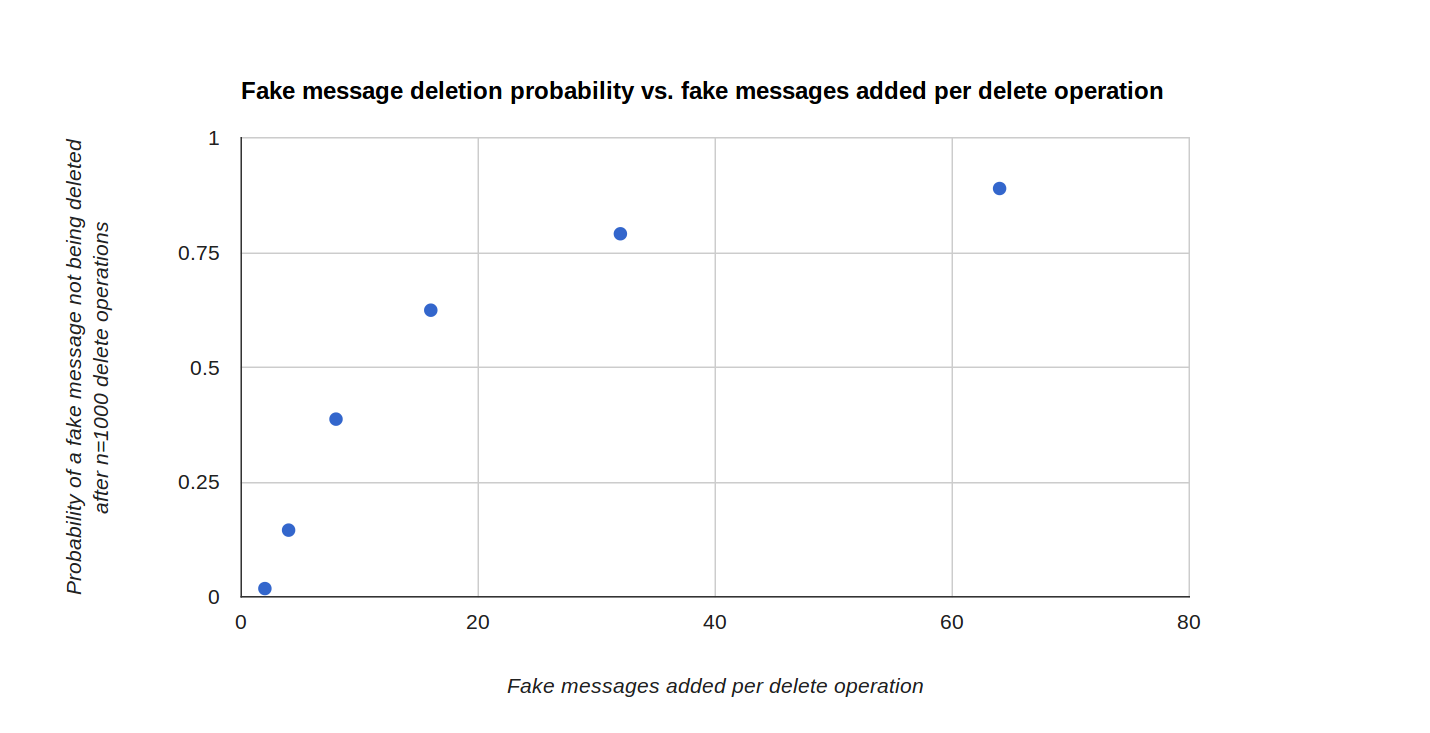
\includegraphics[width=\textwidth]{fake-message-deletion-probability-vs-num-fake-messages-added}

In this case, we need an $f$ of 64 to achieve merely a $p=0.89$ that a fake message is not deleted (compare, of course, with $p=1$ for a real message under the assumption that no real messages are ever deleted).

Is this feasible? Certainly with no space constraints, it is, but we must also consider this solution under reasonable constraints. Gmail, a popular email provider, allots 17 GB of space to a user. Assume that a user wants to use this email address for 5 years (a conservative estimate), and that messages average 170 kB (this number is accurate for my personal email account). Then, 100,000 messages will fit into the server. Say that we are comfortable with having 32 fake messages uploaded per delete operation. Even discounting other messages received in the mail server, this only allows 3125 delete operations, which amounts to 1.7 delete operations per day over the five years. This amount to a delay of about 7 hours any time the user would like to delete a message \--- and this is not taking into account the space that real messages will use. While a user without space constraints could certainly choose this method, we will now describe a more feasible solution.

\subsubsection{Mixing}
We can achieve metadata security while constraining mail server growth to a rate roughly consistent with the number of received messages. To do this, \project implements a mixing mechanism whereby scheduled updates push and pull not only a single message, but multiple messages among which the true target message will be disguised.

On a scheduled timer tick with action UP, \project selects MIX NUMBER messages from all messages with an entry in the current INDEX, (those being the messages that exist in CRYPTOBLOBS). It then FETCHes those messages from the server, reassigns their UNIQUE SUBJECTs, reuploads the new messages to the server, then deletes the messages that were fetched. When the messages are reuploaded, the new message is randomly inserted in with them, indistinguishable from the other messages. On a DOWN operation, a similar mixing occurs. MIX NUMBER + 1 messages are selected at random. If the message to be deleted is not among them, one of the selected messages is replaced with the message to actually be deleted. \project then fetches all MIX NUMBER + 1 messages, reassigns UNIQUE SUBJECTs, reuploads the MIX NUMBER messages that are not actually marked for deletion, then deletes all chosen messages. If there are fewer than MIX NUMBER messages to choose from, all existing messages are mixed.





\section{Prototype Client}

% \section{Performance}
% \subsection{Scheduler}


\section{Attacks and Countermeasures}
\subsection{Multiple Client Signup INDEX Rollback}
\begin{enumerate}
\item Client A signs up and makes changes such that the SEQUENCE NUMBER is 10.
\item The IMAP server rolls back the entire system to when the SEQUENCE NUMBER was 8.
\item Client B signs up and accepts that the initial sequence number is 8.
\item Client B makes changes such that the SEQUENCE NUMBER is 12.
\item Client A connects to the server, sees that the sequence number is 12 (which is greater than 10), and accepts the INDEX. Client A assumes that Client B made changes that undid the results of INDEXes 9 and 10 before applying updates 11 and 12.
\end{enumerate}

\subsubsection{Defense}
When a new client signs up, either manually inspect the contents to ensure that they are in the expected state or display the current sequence number on both an existing client and the new client for a user to compare.

\section{Dissemination Considerations}
As discussed in Section~\ref{architecture}, every client of an IMAP server must upgrade to \project if any client does so. Therefore, for this technology to spread, \project must be available across platforms on initial release, as a standard modern user expects to be able to check his or her email across devices and email clients. 

\section{Summary}

\section{Honor Code}
\label{honorcode}
I pledge my honor that this thesis represents my own work in accordance with Princeton University regulations.

\pagebreak

\bstctlcite{bstctl:etal, bstctl:nodash, bstctl:simpurl}
\bibliographystyle{IEEEtranS}
\bibliography{references}

\end{document}







